%!TEX root = comps_NKasimov.tex
\chapter{New Volume Penalization Methods}
\label{chapter:3}
\section{Brinkman-like Penalization for Low Fidelity Simulations}
Due to the coarse grid used in Lo-Fi simulations slightly modified BP methods was developed, in order to match drag force that drives particles obtained numerically with experimental results. The idea is to introduce momentum penalization term which is quadratic in velocity
\begin{align}
\frac {\pt \rho u_i}{\pt t} &= RHS - \frac \chi \eta \rho \rbr{u_i - U_i^o}^2.
\end{align}
From one hand, it forces the solution to the proper value at the obstacle boundary even faster than in case of simple BP, on the other hand this expression makes modeling of the penalization easier and flow independent. Namely, 
\begin{align}
F_{drag} &= \int\displaylimits_\Omega \frac 1 \eta \rho \rbr{u - U^o}^2\ dV \sim \int \displaylimits_A \frac 12 \rho C_d \rbr{u - U^o}^2\ dA, \label{eq:lofi-penal}
\end{align}
where $\Omega$ is the volume of the obstacle, and $A$ is largest cross section are across the flow and $\chi$ is dropped since integration is performed only inside of the obstacle. For the sake of simplicity, let us consider uniform flow around triaxial ellipsoid with semi axes $a,b$ and $c$. In that case $\Omega = \pi a b c$ and $A = \pi a b$, under the assumption that flow goes along $c$ semi axis. So, \eqref{eq:lofi-penal} simplifies into
\begin{align}
\frac {\pi a b c}\eta \sim \frac 12 \pi a b\ C_d \implies \eta \sim \frac c{2C_d}.
\end{align}

\section{Characteristic Based Volume Penalization}
First VP method used in Hi-Fi simulations was Brinkman Penalization. For testing purposes 1D Riemann problem for Euler equations were solved (see Fig.~\ref{fig:riemann_euler}).
\begin{figure}[h!]
\centering 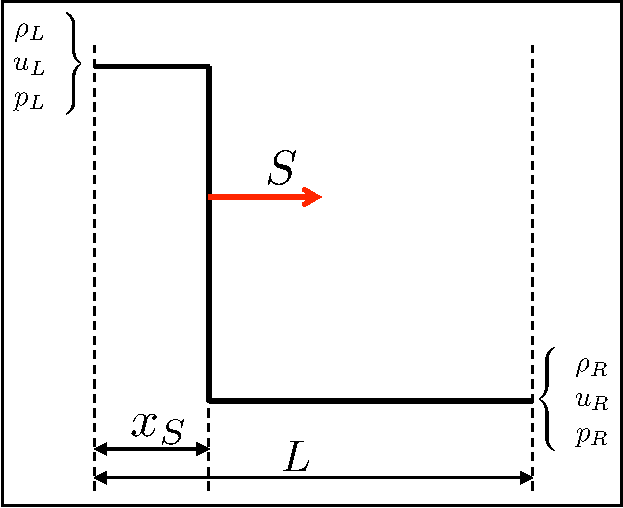
\includegraphics[scale=0.5]{fig/Riemann_Euler.pdf}\\
\caption{Riemann problem set up \label{fig:riemann_euler}}
\end{figure}

To compare results, first, normal self-sustained shock problem was solved with reflection on the right domain boundary. Then right domain was extended and part of the domain was considered as solid obstacle and BP was used to model that solid obstacle/wall. Results revealed that using BP without any modification to supersonic flow leads to significant numerical errors such as phase lag and amplitude error, e.g. pressure seepage (see Fig.~\ref{fig:plain_bp}).
\begin{figure}[h!]
\begin{minipage}{0.49\linewidth}
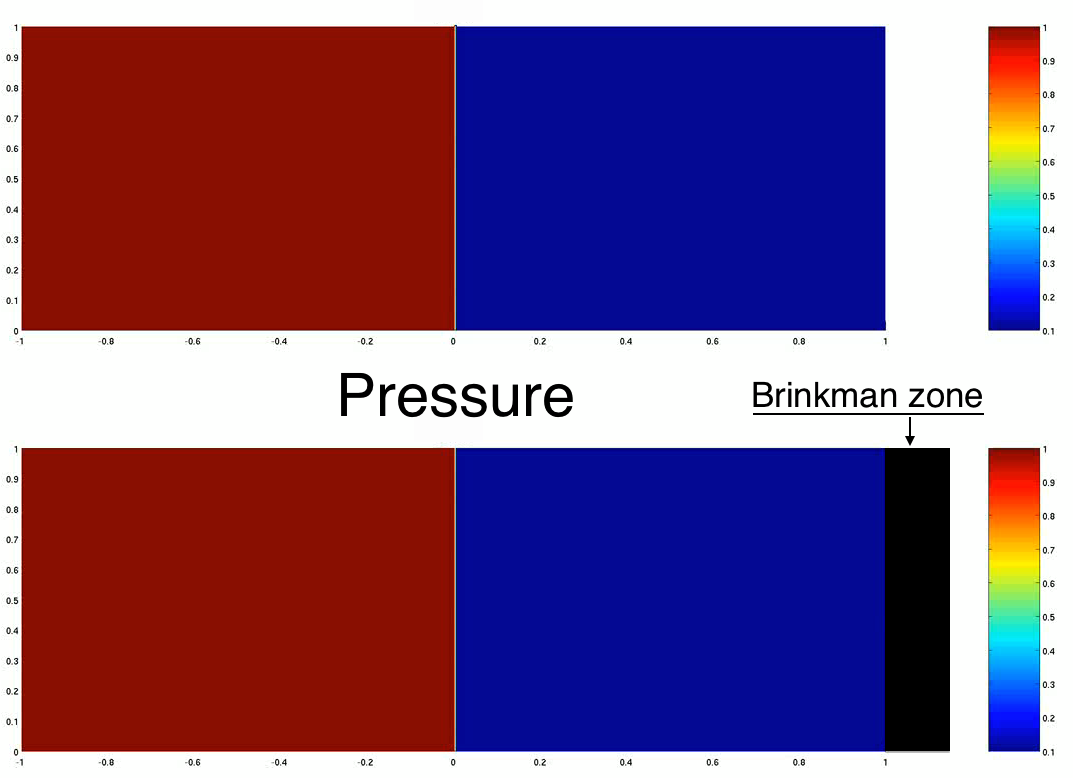
\includegraphics[scale=0.2]{fig/sod1_init.png}\\
\centering{a) Initial condition of SOD1 test}
\end{minipage}
\hspace{0.02\linewidth}
\begin{minipage}{0.49\linewidth}
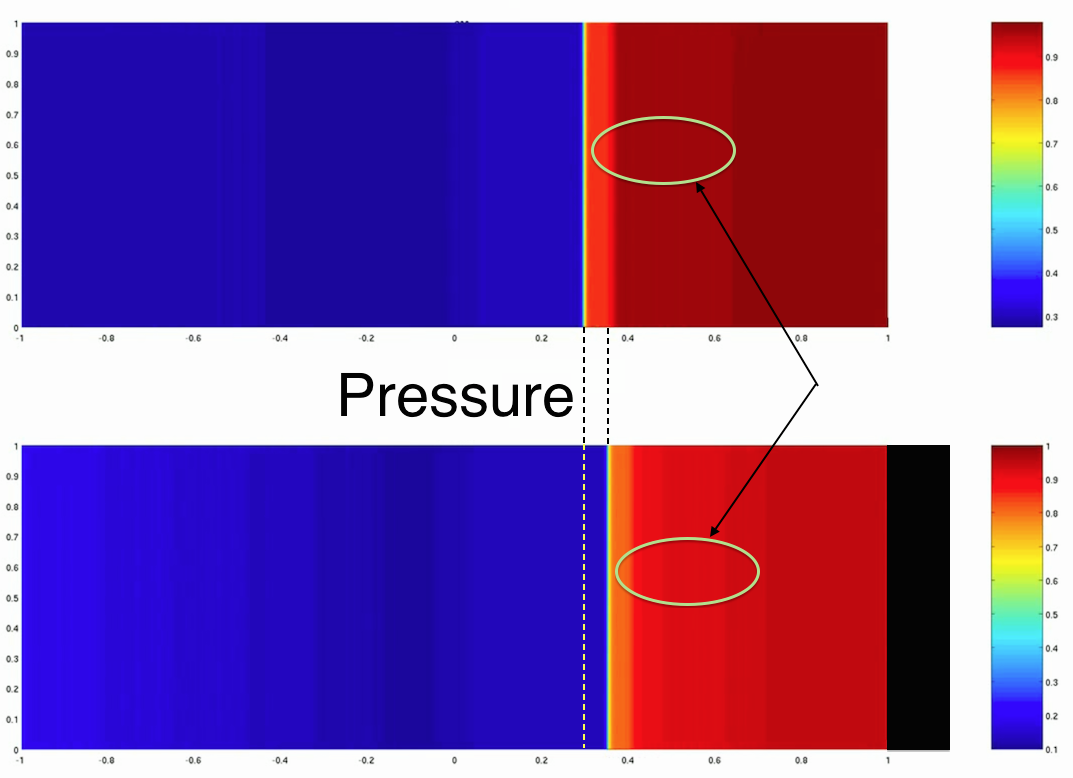
\includegraphics[scale=0.2]{fig/sod1_end.png}\\
\centering{b) End state of SOD1 test}
\end{minipage}
\caption{Normal reflection from the wall (top) and BP (bottom)} \label{fig:plain_bp}
\end{figure}

In order to overcome deficiencies of BP regarding flow regimes and boundary conditions, new VP method was developed. Let us consider general BC that one wants to mimic at the fluid-solid interface
\begin{align}
\mathcal L \rbr \bullet = f_{boundary},
\end{align}
where $\rbr \bullet$ may stand for any of the integrated variables, and operator $\mathcal L$ can describe either Dirichlet or Neumann boundary conditions, or Robin type BC. The idea is to replace evolution problem under the consideration as follows:
\begin{align}
\frac {\pt \phi}{\pt t} = RHS \longrightarrow \frac {\pt \phi}{\pt t} = (1-\chi)RHS - \frac \chi \eta \sbr{\mathcal L \rbr \phi - f_{boundary}}. \label{eq:CBVP}
\end{align}
Obviously, BP method is a special case of CBVP, when $\mathcal L = \mathds 1$ and $f_{boundary} = U^o$ for velocity or $f_{boundary} = T^o$ for temperature. Let us consider the same Riemann problem, but using the following BC at the obstacle instead:
\begin{align}
\fbrr{\begin{array}{rl}
\vbr{u_i^n}_{\pt \Omega} &= U_i^{on} \\ [1ex]
\ds \vbr{\frac {\pt u_i^\tau}{\pt n}}_{\pt \Omega} &= 0 \\ [2ex]
\ds \vbr{\frac {\pt p}{\pt n}}_{\pt \Omega} &= 0
\end{array}},
\end{align}
where $u^n_i = u_j n_j n_i$ is a normal component of the velocity, $u_i^\tau = u_i - u_i^n$ is a tangental component and $\pt / \pt n \equiv n_j \pt / x_j$ is a derivative in normal direction.

According to \eqref{eq:CBVP} evolution equations need to be changed as described below:
\begin{align*}
\fbrl{\begin{array}{rl}
\ds \frac {\pt u_i^n }{\pt t} & = \ds (1-\chi)RHS - \frac \chi {\eta_b} \rbr{u_i^n - U_i^{on}} \\
\ds \frac {\pt u_i^\tau}{\pt t} & = \ds (1-\chi) RHS - \frac \chi {\eta_c} \frac {\pt u_i^\tau}{\pt n} \\
\ds \frac {\pt p}{\pt t} & = \ds (1-\chi) RHS - \frac \chi {\eta_c} \frac {\pt p}{\pt n},
\end{array}}
\end{align*}
which can be translated to the equations in terms of integrated variables (with omitted outside-of-the-obstacle part),
\begin{align}
\fbrl{\begin{array}{rl}
\ds \frac {\pt \rho}{\pt t} & = \ds -\frac 1 {\eta_c} \frac {\pt \rho}{\pt n} \\ [1ex]
\ds \frac {\pt \rho u_i^n}{\pt t} & = \ds -\frac 1{\eta_b} \rho \rbr{u_i^n - U_i^{on}} + \nu_n \gD u_i^n \\ [1ex]
\ds \frac {\pt \rho u_i^\tau}{\pt t} & = \ds -\frac 1{\eta_c} \frac {\pt \rho u_i^\tau}{\pt n} \\ [1ex]
\ds \frac {\pt \rho e}{\pt t} & = \ds -\frac 1{\eta_c} \frac {\pt \rho e}{\pt n} - \frac 1{\eta_b}\rho u_j^n \rbr{u_j^n - U_j^{on}} + \frac 1{\eta_c} u_j^n \frac {\pt \rho u_j^n}{\pt n} + u_j^n \nu_n \gD u_j^n.
\end{array}} \label{eq:CBVP_euler}
\end{align}
One can notice that in \eqref{eq:CBVP_euler} there are extra terms in energy equation. They appear due to the fact that there is no so called ``characteristic term'' in normal momentum penalization and one need to add it and subtract in order to have characteristic term in energy equation as well. Also, extra diffusive term was added to the same normal momentum equation to enhance stability. These technique resulted improvements in comparison to regular BP method (see Fig.~\ref{fig:sod_cbvp}). One can find more results on using CBVP for variety of problems in Chapter 4, as well as benchmarks.
\begin{figure}[h!]
\centering 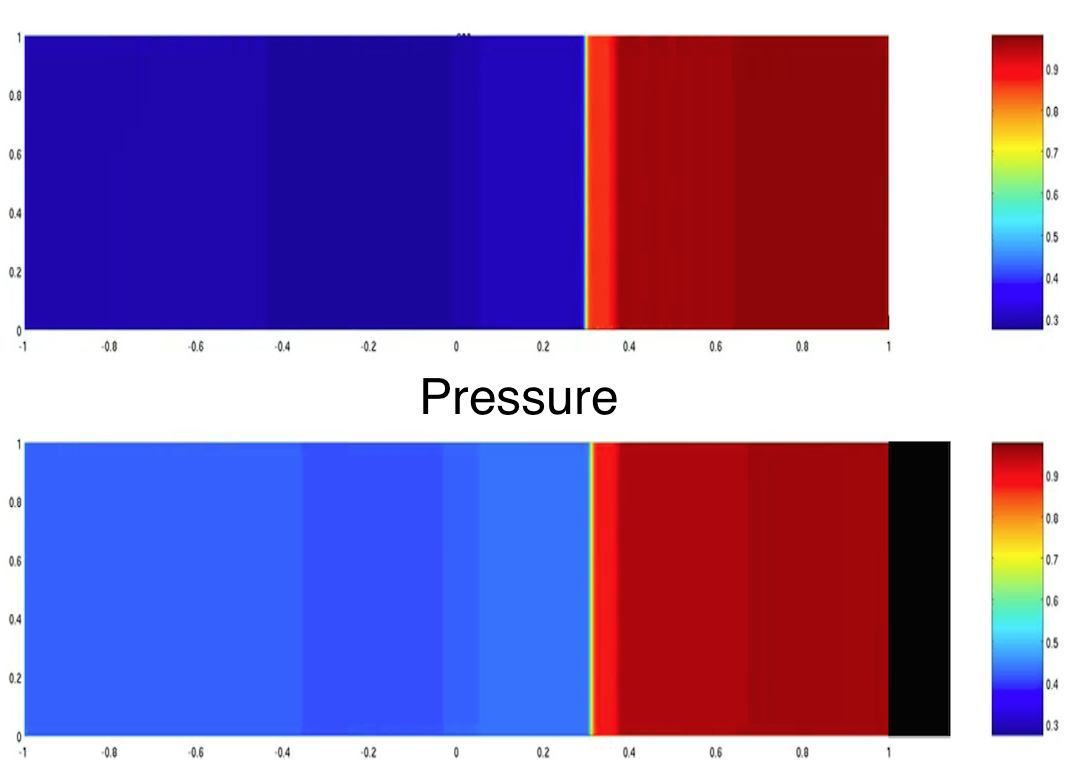
\includegraphics[scale=0.3]{fig/sod1_cbvp.png}\\
\caption{SOD1 test problem with CBVP \label{fig:sod_cbvp}}
\end{figure}







